\chapter{Requirements Specification}

\section{Introduction}
Throughout this chapter, we specify both the functional and non-functional requirements, identify the system actors, and present the global use case diagram.
By defining these elements, we aim to establish a clear and shared understanding of the system’s expected behavior and constraints, providing a solid foundation for the subsequent design and implementation phases.

\section{Functional Requirements}
Functional requirements define \emph{what} the system should perform. The main functionalities of our system are as follows:

\vskip0.5cm
— Authenticate;
\vskip0.2cm
— View Dashboard;
\vskip0.2cm
— View Statistics summary;
\vskip0.2cm
— Trigger Network Analysis;
\vskip0.2cm
— View Alerts List;
\vskip0.2cm
— View Reports;
\vskip0.2cm
— Analyze Network Flow;

\section{Non-Functional Requirements}

Non-functional requirements define \emph{how} the system should perform its functions. They describe the quality attributes and constraints of the system:

\vskip0.4cm
\textbf{Performance:} The system must process network traffic and generate analysis results with minimal latency, ensuring fast detection of potential intrusions.

\vskip0.3cm
\textbf{Security:} The system must ensure secure authentication and enforce role-based access control, preventing unauthorized actions and protecting system integrity, while supporting non-repudiation to guarantee accountability and traceability of all operations.

\vskip0.3cm
\textbf{Reliability:} The system must perform its functions consistently, handle errors gracefully, and ensure that failures are detected and managed without disrupting overall operation.

\vskip0.3cm
\textbf{Maintainability:} The system should be easy to maintain, allowing for efficient debugging, updates, and modifications to existing components.

\vskip0.3cm
\textbf{Extensibility:} The system should support the addition of new features, such as new detection models or data sources, without requiring major redesign.

\vskip0.3cm
\textbf{Availability:} The system must be accessible and operational whenever needed, minimizing downtime and ensuring continuous monitoring of network activity.

\vskip0.3cm
\textbf{Usability:} The system should provide an intuitive interface, enabling users to efficiently navigate and interact with its functionalities.

\section{Actors Identification}
Actors are external entities, users, organizations, or external systems that interact with the system to achieve one or more functional requirements, with each actor representing a specific role.
\vskip0.05cm
In the context of our project, we identify three primary actors illustrated in Figure~\ref{fig:actors}
\vspace{-0.5cm}
\begin{figure}[h!]
    \centering
    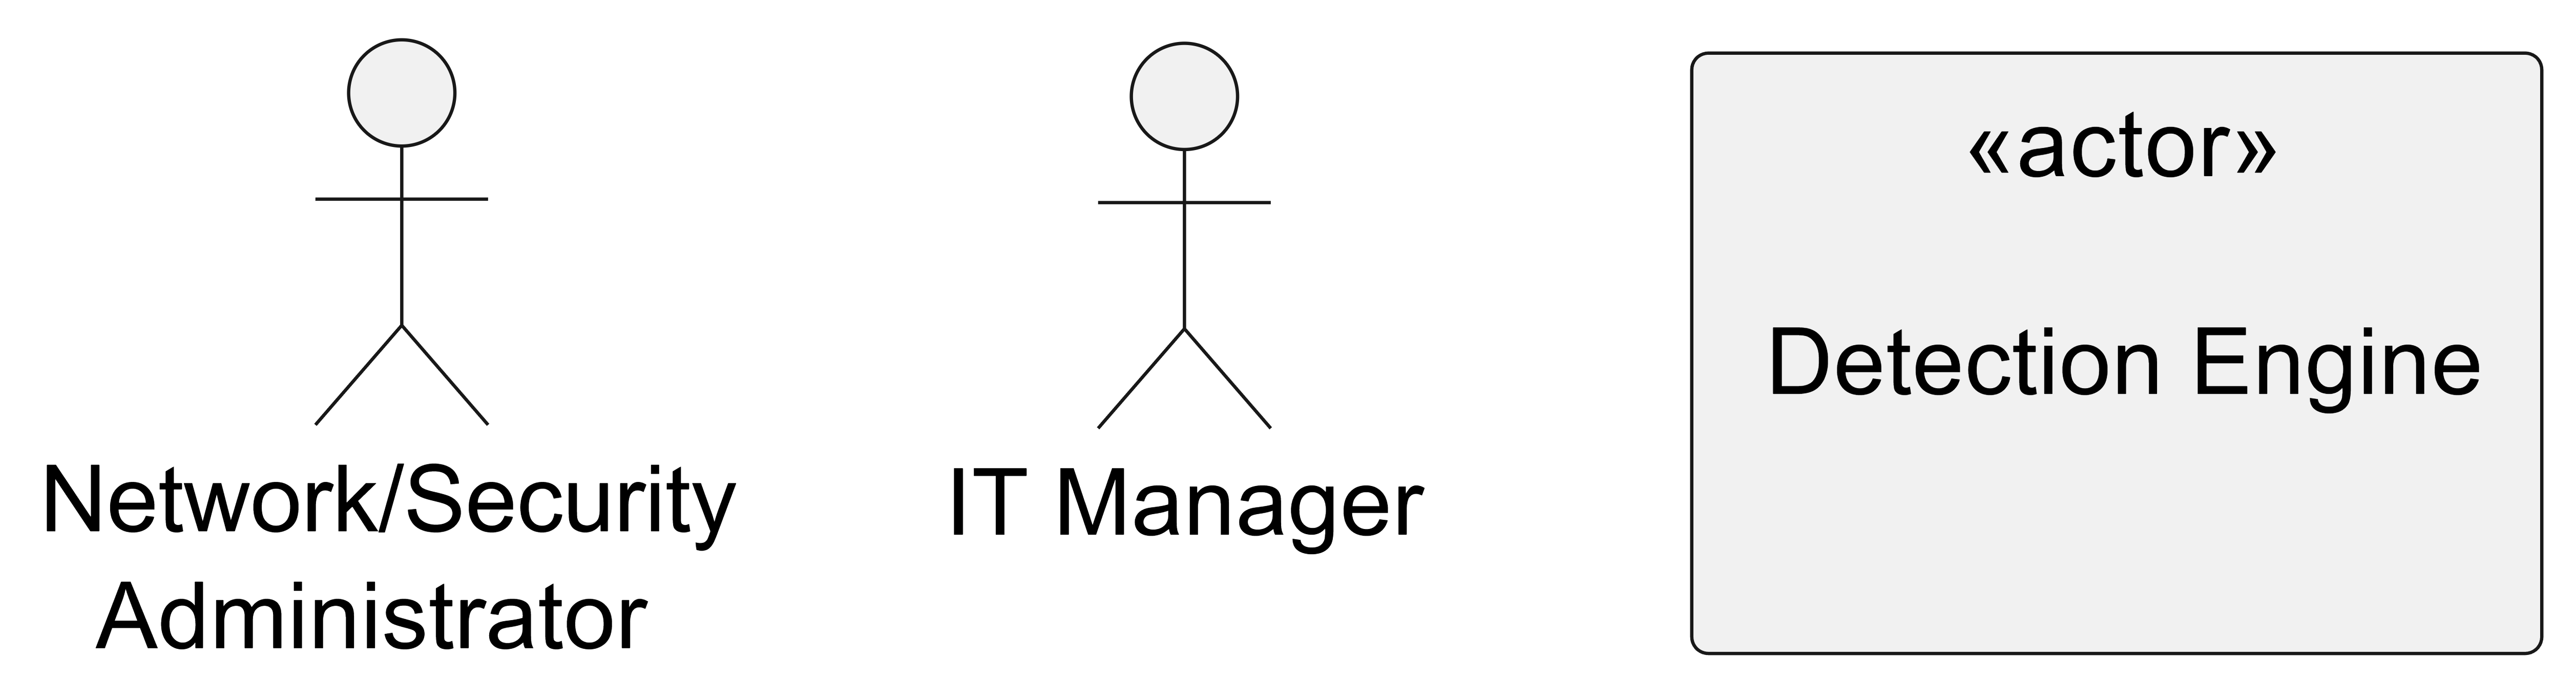
\includegraphics[width=1\columnwidth]{../diagrams/actors.png}
    \caption{Actors}
    \vspace{-0.5cm}
    \label{fig:actors}
\end{figure}
\vskip0.1cm
Table~\ref{tab3} presents the roles of each actor in our system.
\vspace{-0.1cm}
\begin{table}[H]
    \begin{center}
        \caption{Roles of Actors}
        \label{tab3}
        \begin{tabular}{|l|>{\raggedright\arraybackslash}p{6cm}|}
            \hline
            \rowcolor[gray]{0.8}\bfseries Actor & \bfseries Role             \\
            \hline
            Network/Security                    & - Authenticate             \\
            Administrator                       & - View Dashboard           \\
                                                & - View Statistics Summary  \\
                                                & - Trigger Network Analysis \\
                                                & - View Alerts List         \\
            \hline
            It Manager                          & - Authenticate             \\
                                                & - View Dashboard           \\
                                                & - View Statistics Summary  \\
                                                & - View Reports             \\
            \hline
            Detection Engine                    & - Analyze Network Flow     \\
            \hline
        \end{tabular}
    \end{center}

\end{table}
\newpage
\section{Use Case Diagram}
A use case diagram is a visual representation of \emph{how} users interact with the system and \emph{what} a system does through different use cases.
Figure~\ref{fig:use_case} illustrates that diagram.
\begin{figure}[h!]
    \centering
    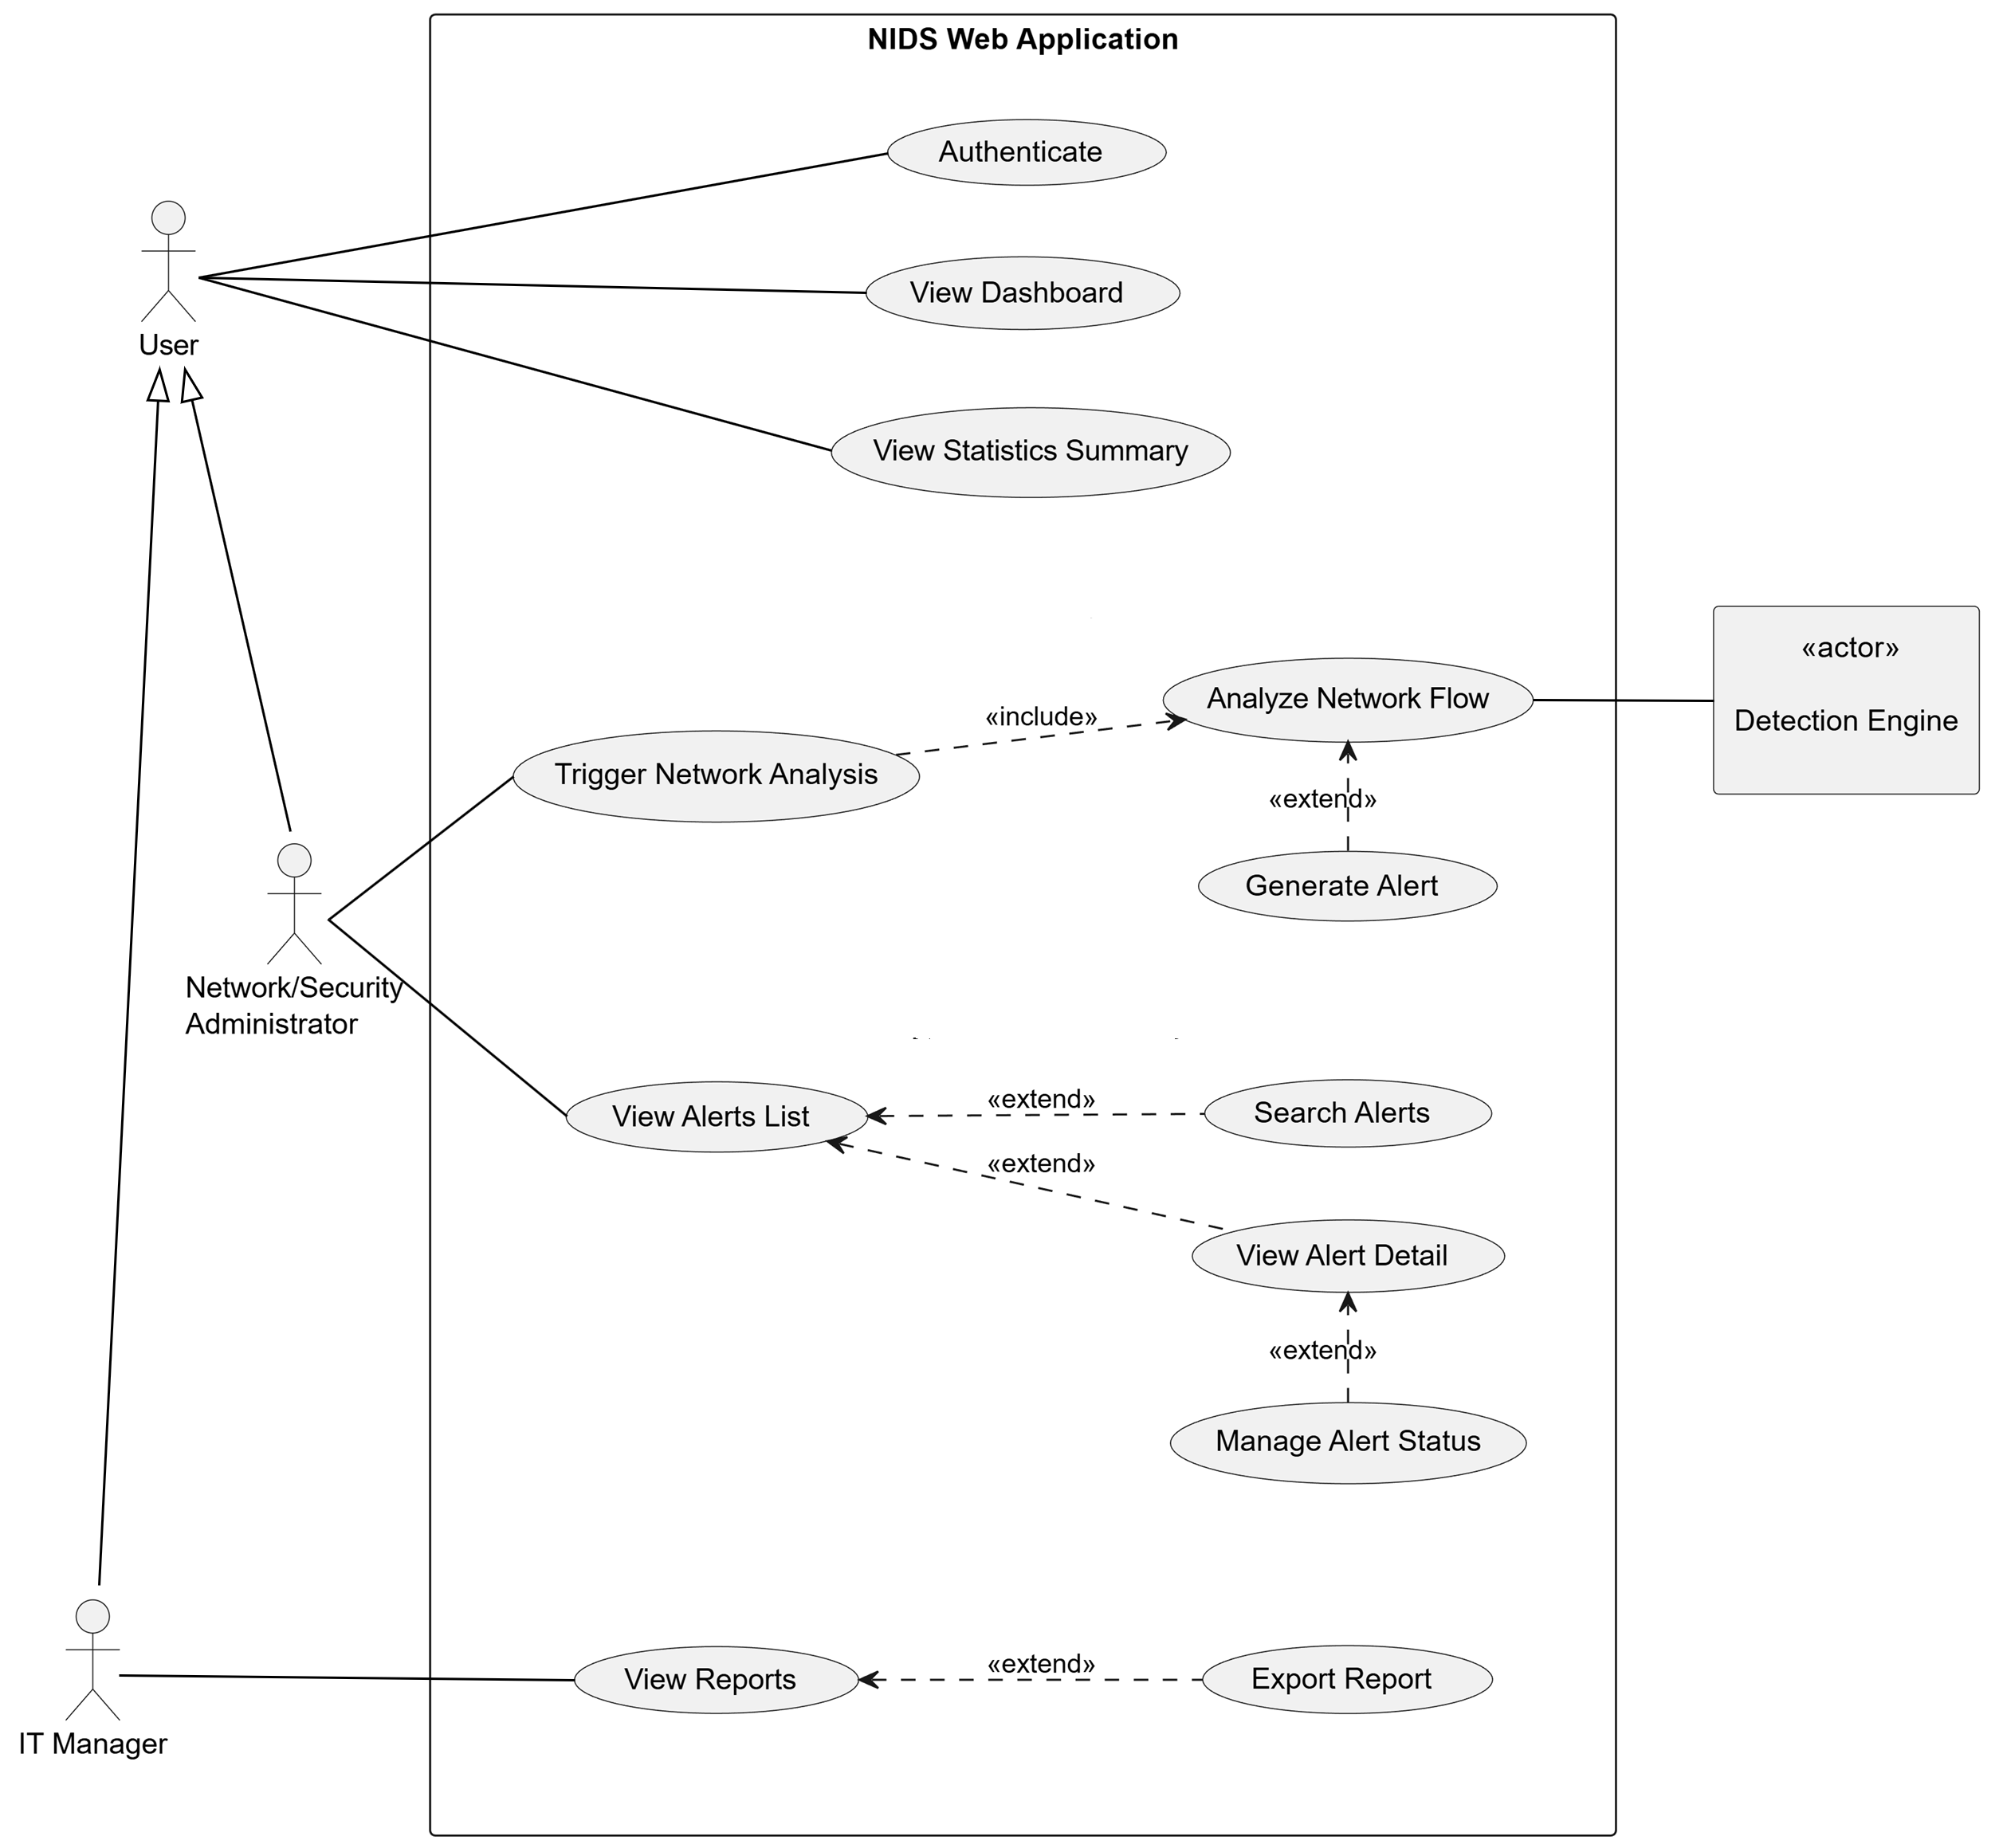
\includegraphics[width=1\columnwidth]{../diagrams/use-case.png}
    \caption{Use Case Diagram}
    \label{fig:use_case}
\end{figure}

\section{Conclusion}
In this chapter, we outline the functional and non-functional requirements of our system, identify the primary actors, and represent the way they interact with the system and the system's functionality via a use case diagram. In the next chapter, we present the conceptual design of the platform.